\documentclass [letterpaper, 12pt] {article}
\usepackage[margin=1in]{geometry}
\usepackage{graphicx, subcaption, ragged2e}
\usepackage{amsmath}
\usepackage{epsfig}
\usepackage{parskip}
\usepackage[utf8]{inputenc}
\usepackage[english]{babel}
\usepackage{cite}
\usepackage{float}

\graphicspath{{../Figures/}{../Images/}}

\begin{document}

\begin{titlepage}
	\centering
	\vspace*{\fill}

	\vspace*{0.5cm}

	\huge\bfseries
	A Data-driven Comparison of Plague Models

	\vspace*{0.5cm}

	\large Luke Mattfeld

	\vspace*{\fill}
\end{titlepage}

\pagenumbering{roman}
\tableofcontents
\newpage
\pagenumbering{arabic}

\section {Abstract}

Transmission methods for \textit{Yersinia pestis}-based plagues in historical accounts, the most well known being the Black Death or Bubonic plague, has long been speculated. Due to the lack of medical technology of the time and the vast number of deaths, little is certainly known. Here, we extend the work of Dean et al.\ in the PNAS article "Human ectoparasites and the spread of plague in Europe during the Second Pandemic" in comparing proposed transmission models to historical death data. This is done by using the Markov-Chain Monte-Carlo method to estimate unknown parameter distributions for a given model on a dataset, and comparing the fit across models. In addition to the 3 models tested by Dean et al., we compare a new Rat-Flea Transmission model developed by EWU fellow Ian Lynch. Our results indicate that this new model is comparably performant to the best model proposed by Dean et al., which suggests that rat-flea transmission is plausible for the datasets examined.

\pagebreak

\section {Introduction}

The Plague has devastated populations and greatly affected human history in its 3 major outbreaks. These outbreaks include the Justinian Plague, the Bubonic Plague, and the more recent outbreak in the 1800’s in China \cite{barbara_et_al_2016}.
The driving force of the plague is the bacteria Yersinia Pestis, which manifests in 3 primary infection types: bubonic, pneumonic, and septicaemic \cite{DITCHBURN201965}.

Bubonic plague, the most well-known, manifests in painful, swollen “Buboes” at or near the lymph nodes. It is spread through contact with the skin, in most cases insect bites. The mortality rate for untreated bubonic plague is 40-70\% \cite{ditchburn_hodgkins_2019} . Pneumonic plague, also fairly deadly, is spread through aspirated bacteria, and starts in the lungs. It is spread through aspiration in the presence of infected individuals or in an environment laiden with the bacteria. The mortality rate for untreated pneumonic plague is ~90-95\% Finally, there is a septicaemic plague which is the most deadly. Incubation for septicaemic is veryfast, and spreads fast throughout the body. Some reports said infected individuals would feel fine in the morning and be dead by evening. This had little effect on the overall epidemic when compared to the Bubonic and Pneumonic plagues, only accounting for 10-15\% of all cases of the plague since people would tend to die before they had time to develop other symptoms or methods of spreading. For this reason, the septicaemic plague will not be used in this research. The mortality rate for untreated septicaemic plague is 100\% \cite{ditchburn_hodgkins_2019}.

While historical evidence contains many details as to how the various outbreaks of the Plague have affected society, art, and culture, much less is known and is certain about the way in which the plague spread. The state of medical technology at the time has led to speculation and deductive reasoning from the available data. From this the currently accepted theory has been formed: The Bubonic plague was mostly spread through the interaction of rat and flea populations. The fleas host the disease contracted through biting a host. The fleas then are carried by the rats, which are not significantly affected by the disease. Once a carrying capacity for the rat has been reached, the flea is forced to find another host. Due to the nature of the bacteria, the digestive tract of the flea is “clogged up” (better alliteration needed) and the flee is pushed to constant biting due to hunger. The flea then regurgitates the bacteria into the many open bites. In this way the bacteria enters the new host.

Specifically when examining the second outbreak, the poor hygienic conditions in Europe at the time, the presence of rats and fleas in and around human habitation was common. Thus, when infected rats arrived through trade routes and incoming ships, the population was quickly infected.
The exact role of the pneumonic plague is somewhat unknown. It does, under certain conditions, form from an existing case of bubonic plague, and is then spread as pneumonic from that point on. Some records of death rates are in areas and at rates which would be explained better by the spread of this pneumonic type. However, the lack of medical knowledge at the time fails us here.
This theory is partially supported by historical evidence - as sightings of sick rats were observed, and were thought to bring “bad air” which was the source of new infection. In addition ships began to be refused at many ports in Europe due to the infection they carried via the rats and sailors \cite{barbara_et_al_2016}.

However Dean et. al.\ in a recent modeling study suggest otherwise \cite{Dean1304}. In this paper, Dean et al.\ investigates several mechanisms of spread likely to be responsible for historic plague events. They accomplished this by fitting the various differential models of plague spread (Rat-flea, pneumonic, and  a new human-ectoparasite model) to historical death data. Their results suggested that the new human-ectoparasite model better fit the death curve for 7 out of 9 datasets from various cities.

%\pagebreak
%
%\section {Background}


\pagebreak

\section {Preliminary Models}
This paper's seminal work by Dean et al.\ \cite{Dean1304} set out to compare 3 models of
transmission: 2 for bubonic and 1 for pneumonic plague. The rat-flea-transmission (RFT) model used was obtained from two papers by Keeling and Gilligan \cite{keeling_gilligan_zoonosis} \cite{keeling2000}, and going forward will be referred to as the Keeling-Gilligan model. While in the Dean work the Keeling-Gilligan rat-flea model did not perform as well as the Human-ecto model, a new RFT model has recently been proposed. This model developed by Lynch and Oster \cite{lynch-plague-modeling} , hereafter known as the Lynch-Oster model, takes a different model structure to that of Keeling and Gilligan. These models, taken from their respective papers, are as such:

\subsection {Pneumonic Model}
Direct human-to-human transmission, modeled with three differential equations. Since so few recovered from the pneumonic plague, the population follows a simple SID model
(Susceptible, Infected, Dead.):

\begin{figure}[H]
	\centering
	
\includegraphics[width=0.5\linewidth]{sid-graph.png}
	\caption{SIR Model Diagram}
\end{figure}


\begin{align}
	\frac{dS_h}{dt} & = - \beta_p \frac{S_h I_h}{N_h}              \\
	\frac{dI_h}{dt} & = \beta_p \frac{S_h I_h}{N_h} - \gamma_p I_h \\
	\frac{dD_h}{dt} & = \gamma_p I_h
\end{align}

Given the high mortality rates of Pneumonic plague, for these relatively small datasets it will be considered 100\% lethal.

\newpage
\subsection {Keeling-Gilligan Rat Model}
This model of rat-flea-human transmission is modeled with ten differential equations. Given that fleas live on the rats, they are modeled as an average number of fleas per rat H, and the number of infections fleas not on rats F:

\begin{align}
	\frac{dH}{dt} & = r_f H \left( 1 - \frac{H}{K_f} \right) \\
	\frac{dF}{dt} & = (1 - g_r) \gamma_r I_r H - d_f F
\end{align}

The Rat and Human populations follow an SIRD model (Susceptible, Infected, Recovered, Dead):

\begin{figure}[H]
	\centering
	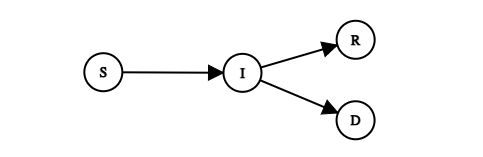
\includegraphics[width=0.65\linewidth]{sird-graph.png}
	\caption{SIRD Model Diagram}
\end{figure}

\begin{align}
	\frac{dS_j}{dt} & = - \beta_r \frac{S_j F}{N_j} \left[ 1 - e^{-aN_r} \right]              \\
	\frac{dI_j}{dt} & = \beta_r \frac{S_j F}{N_j} \left[ 1 - e^{-aN_r} \right] - \gamma_j I_j \\
	\frac{dR_r}{dt} & = g_j \gamma_j I_j                                                      \\
	\frac{dD_r}{dt} & = (1 - g_j) \gamma_j I_j
\end{align}

Here, j = r, h for rats and humans respectively

In this case, the total of population j is $T_j = S_j + I_j + R_j$.

\newpage
\subsection{Lynch-Oster Rat Model}

These equations govern the dynamics of the rats and fleas with logistic models:

\begin{align}
	\frac{dR_T}{dt} & = (\frac{\beta_R}{K_R})R_T(K_R-R_T)-\delta R_c                                             \\
	\frac{dR_c}{dt} & = \alpha \frac{F_c}{F_T} (R_T-R_c)-\frac{\beta_R}{K_R}(R_T)(R_c) - \delta R_c - \gamma R_c \\
	\frac{dF_T}{dt} & = (\frac{\beta_F}{K_F})F_T(K_F-F_T)-\rho F_T                                               \\
	\frac{dF_c}{dt} & = \lambda \frac{R_c}{R_T} (F_T-F_c) - \rho F_c
\end{align}

Here $R_t$ indicates the total population of rats and $R_c$ indicates the number of contaminated rats. The equations for the fleas follow similarly.

The human dynamics follow an SEIR model (Susceptible, Exposed, Infected, Recovered, Dead) where the inflow to the infected state depends on the
population density of the contaminated fleas and an interaction term for the two populations.
\vspace{-0.2cm}
\begin{figure}[H]
	\centering
	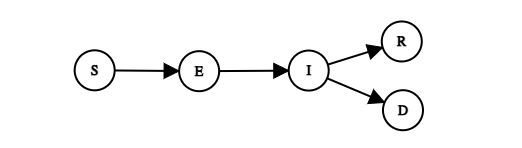
\includegraphics[width=0.75\linewidth]{seird-graph}
	\vspace{-0.5cm}
	\caption{SEIR Model Diagram}
\end{figure}
\vspace{-0.5cm}

\begin{align}
	\frac{dS}{dt}   & = \beta (S+R_b) - \sigma S \frac{F_c}{F_T} - \mu S \\
	\frac{dE}{dt}   & = \sigma S \frac{F_c}{F_T} - \nu E - \mu E         \\
	\frac{dI}{dt}   & = \nu E - \phi I - rI                              \\
	\frac{dR_b}{dt} & = rI - \mu R_b                                     \\
	\frac{dD}{dt}   & = \phi I + \mu N_h
\end{align}

Note that the diagram and set of equations technically model an SEIRD model (adding death). While the Lynch-Oster RFT model did account for deaths in the SEIR dynamics, it did not have a term for counting deaths. This was formulated by accounting for the intrinsic death of the total population $N$, as well as the deaths from infected individuals due to the plague.

\subsection {Human-Ectoparasite Model}
Human-parasite transmission is modeled with seven differential equations.

Here, the parasite modeled is lice, which follows an SI model (Susceptible, Infected):

\begin{figure}[H]
	\centering
	\includegraphics[width=0.55\linewidth]{sI-graph}
	\caption{SEIR Model Diagram}
\end{figure}

\vspace{-0.2cm}

\begin{align}
	\frac{dS_l}{dt} & = r_l S_l \left( 1 - \frac{N_l}{K_l} \right) - \left[ \left( \beta_{low} I_{low} + \beta_{high} I_{high} \right) \frac{S_l}{N_h} \right] \\
	\frac{dI_l}{dt} & = \left[ \left( \beta_{low} I_{low} + \beta_{high} I_{high} \right) \frac{S_l}{N_h} \right] - \gamma_l I_l
\end{align}

The human population follows an $S I_l I_h R D$ model (Susceptible, Infected (low), Infected (high), Recovered, Dead):

\begin{figure}[H]
	\centering
	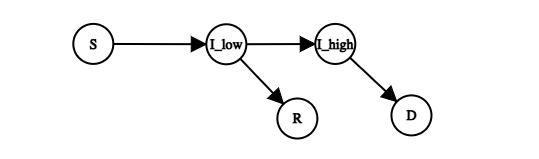
\includegraphics[width=0.75\linewidth]{siird-graph.png}
	\caption{SIIRD Model Diagram}
\end{figure}

\begin{align}
	\frac{dS_h}{dt}      & = -\beta_l \frac{S_h I_l}{N_h}                   \\
	\frac{dI_{low}}{dt}  & = \beta_l \frac{S_h I_l}{N_h} - \sigma_b I_{low} \\
	\frac{dI_{high}}{dt} & = (1-g_h) \sigma_b I_{low} - \gamma_b I_{high}   \\
	\frac{dR_h}{dt}      & = g_h \sigma_b I_{low}                           \\
	\frac{dD_h}{dt}      & = \gamma_b I_{high}                              \\
\end{align}

This model includes terms which differentiate between high and low infectiousness of bacteria.

\pagebreak

\subsection{Parameters}
\subsubsection{Table of Parameters for existing models}
Table reconstructed from Dean et. al \cite{Dean1304}
\begin{table}[H]
	\resizebox{\textwidth}{!}{%
		\begin{tabular}{|c|l|l|}
			\hline
			\multicolumn{1}{|c|}{\textbf{Parameter}} & \multicolumn{1}{c|}{\textbf{Value}} & \multicolumn{1}{c|}{\textbf{Definition}}                                        \\ \hline
			\multicolumn{1}{|l|}{\textbf{Humans}}    &                                     &                                                                                 \\
			$\beta_{low}$                            & U(0.001, 0.05)                      & Transmission rate for bubonic plague from mildly infectious humans to body lice \\
			$\beta_{high}$                           & U(0.001, 1)                         & Transmission rate for bubonic plague from highly infectious humans to body lice \\
			$\beta_p$                                & U(0.001, 1)                         & Transmission rate for pneumonic plague                                          \\
			$\beta_h$                                & U(0.001, 0.2)                       & Transmission rate for bubonic plague from rat fleas to humans                   \\
			$\sigma_b^{-1}$                          & 8.0 (d)                             & Average low infectious period for bubonic plague                                \\
			$\gamma_b^{-1}$                          & 2.0 (d)                             & Average high infectious period for bubonic plague                               \\
			$\gamma_p^{-1}$                          & 2.5 (d)                             & Average infectious period for pneumonic plague                                  \\
			$\gamma_h^{-1}$                          & 10.0 (d)                            & Average duration of infection for bubonic plague                                \\
			$g_h$                                    & 0.4                                 & Probability of recovery from bubonic plague                                     \\ \hline
			\multicolumn{1}{|l|}{\textbf{Lice}}      &                                     &                                                                                 \\
			$r_l$                                    & 0.11 (per d)                        & Natural lice growth rate                                                        \\
			$K_l$                                    & 15.0 (per person)                   & Lice index at carrying capacity                                                 \\
			$\beta_l$                                & 0.05                                & Transmission rate for bubonic plague from body lice to humans                   \\
			$\gamma_l^{-1}$                          & 3.0 (d)                             & Average infectious period for bubonic plague                                    \\ \hline
			\multicolumn{1}{|l|}{\textbf{Rats}}      &                                     &                                                                                 \\
			$\beta_r$                                & U(0.001, 1)                         & Transmission rate for bubonic plague from rat fleas to rats                     \\
			$\gamma_r^{-1}$                          & 5.2 (d)                             & Average infectious period for bubonic plague                                    \\
			$g_r$                                    & 0.1                                 & Probability of recovery from bubonic plague                                     \\ \hline
			\multicolumn{1}{|l|}{\textbf{Fleas}}     &                                     &                                                                                 \\
			$r_f$                                    & 0.0084 (per d)                      & Natural flea growth rate                                                        \\
			$K_f$                                    & 6.0                                 & Average number of fleas at carrying capacity                                    \\
			$d_f^{-1}$                               & 5.0 (d)                             & Death rate of fleas                                                             \\
			$a$                                      & 3.0/$S_r(0)$                        & Searching efficiency                                                            \\ \hline
		\end{tabular}%
	}
	\caption{U indicates the range of a uniformly distributed variable. (d) indicates days}
\end{table}


\subsubsection{Table of Parameters for the Lynch-Oster model}

\begin{table}[H]
	\resizebox{\textwidth}{!}{%
		\begin{tabular}{|c|l|l|}
			\hline
			\multicolumn{1}{|c|}{\textbf{Parameter}} & \multicolumn{1}{c|}{\textbf{Value}} & \multicolumn{1}{c|}{\textbf{Definition}}     \\ \hline
			\multicolumn{1}{|l|}{\textbf{Humans}}    &                                     &                                              \\
			$\beta$                                  & U(0.001, 1)                         & Intrinsic birth rate                         \\
			$\sigma$                                 & U(0.001, 1)                         & Chance of becoming infected from flea bite   \\
			$\mu$                                    & U(0.001, 1)                         & Intrinsic death rate                         \\
			$v^{-1}$                                 & U(0.25, 10) (d)                     & Incubation period of the disease             \\
			$r^{-1}$                                 & U(1, 100) (d)                       & Rate of recovery from bubonic plague         \\
			$\phi^{-1}$                              & U(1, 100) (d)                       & Death rate from bubonic plague               \\ \hline
			\multicolumn{1}{|l|}{\textbf{Rats}}      &                                     &                                              \\
			$\beta_R$                                & U(0.1, 1)                           & Intrinsic birth rate for rats                \\
			$K_R$                                    & 1.5 * $N_h$                         & Carrying capacity for rats                   \\
			$\delta$                                 & U(0.001, 1)                         & Death rate from bubonic plague               \\
			$\alpha$                                 & U(0.001, 1)                         & Infectivity of the plague from fleas to rats \\
			$\gamma$                                 & U(0.001, 1)                         & Recovery rate for rats                       \\ \hline
			\multicolumn{1}{|l|}{\textbf{Fleas}}     &                                     &                                              \\
			$\beta_F$                                & U(10, 100)                          & Intrinsic birth rate for fleas               \\
			$K_F$                                    & $6 * K_R$                           & Carrying capacity for fleas                  \\
			$\rho$                                   & U(0.001, 1)                         & Death rate from bubonic plague               \\
			$\lambda$                                & U(0.001, 1)                         & Infectivity of the plague from rats to fleas \\ \hline
		\end{tabular}%
	}
	\caption{U indicates the range of a uniformly distributed variable. (d) indicates days}
\end{table}

Here, most of the parameters for this model are uniformly distributed, since little is known about the physical associations of many of them. The range intrinsic deaths and births was calculated from work by Urlanis on the population growth in Europe \cite{Urlanis}. Prior distribution of parameters provides bounds for possible values based on data, while letting the specific output be determined by the fitting process (See MCMC explanation for details).



\pagebreak

\section{Method: Markov-Chain Monte-Carlo}

The method we will use to compare the effectiveness of these models against real-world data is Markov-Chain Monte-Carlo (MCMC). MCMC is a method of fitting unknown parameters in models to data which follows these models.

\subsubsection{Mone Carlo methods}
MCMC is, as it's name suggests, a Monte Carlo method. To understand MCMC properly, we must understand the concept behind Monte Carlo methods and simulations. This method is used to sample a distribution: specifically when there exists an unknown distribution determined by the value of random variables having some known distribution. A Monte-Carlo method runs many simulations of the underlying behavior that creates this distribution, collecting the outputs. \cite{holmes} This can be used to achieve the probability distribution of that unknown variable, and make predictions on its value in various contexts. This kind of simulation is particularly good at long-term prediction as it "project(s) outcomes farther out in time with more accuracy" as the number of simulation iterations increase. \cite{ibm_cloud_2020}

\subsubsection{Markov Chains}
This particular Monte-Carlo method uses Markov chains to simulate the underlying behavior of these models. A definition of Markov chains is given by Wolfram:

"A Markov chain is collection of random variables ${X_t}$ (where the index t runs through 0, 1, ...) having the property that, given the present, the future is conditionally independent of the past." \cite{weisstein}

Basically, it's a series of computations that only rely on the current state to compute the next.
Markov chains are quite general then, and can be used in many ways. They can be used to model state machines where the next state only depends on the current state and a set of probabilities to the next possible states. They can be used to train predictive models, like next-word prediction given the past n words that's commonly found in predictive keyboards on smartphones. And, in the case of MCMC it can be used to explore the probability distribution space of a parameter in a fitted model.

\begin{figure}[H]
	\centering
	\begin{subfigure}{0.5\textwidth}
		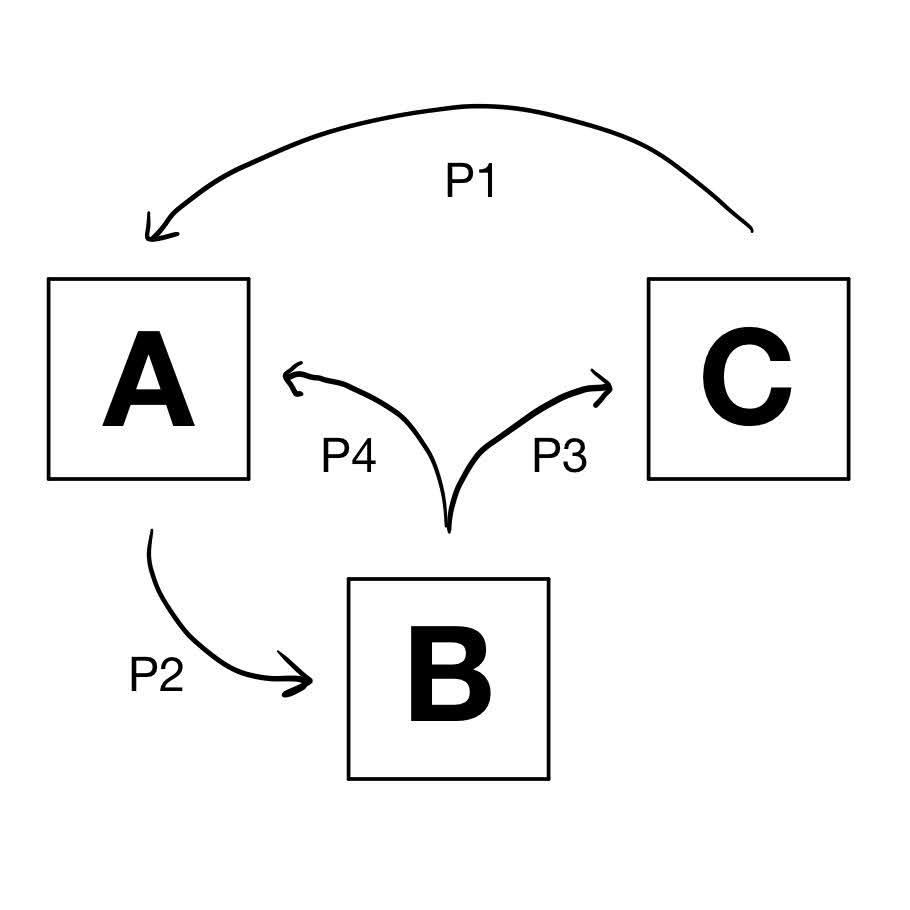
\includegraphics[width=\textwidth]{state_machine.jpg}
	\end{subfigure}
	\caption{Example diagram of a state machine where state change probabilities are determied by the current state and a set of probabilities $\{p_1, p_2, p_3, p_4\}$. A markov chain could model this behavior with each step, or generate these probabilities by modeling the underlying processes.}
\end{figure}

\subsubsection{MCMC}

Putting these to together we get MCMC. It's a Monte-Carlo method which uses Markov chains to generate the parameter sample distributions. By exploring the distribution of each of these parameters, the chains are effectively modeling the behavior of the change a parameter makes in the model given the data.

The exact method of traversing these parameter distributions makes use of Bayesian statistics. Here, the data is king, and all unknowns in the model must be fitted to the data itself - no estimators. So, in bayesian terms what we want to do with MCMC process is, given:
\begin{itemize}
	\item $\vec{\alpha}$ - vector of unknown parameters
	\item $\mathcal{D}$ - data
	\item $\mathcal{M}$ - model
\end{itemize}

We want to find: $P(\vec{\alpha} | \mathcal{D}, \mathcal{M})$. This is the probability, or distribution, of these unknown parameters, given the data and model. It's known as the Posterior distribution, or what you consider the probability of your parameters to be \textit{post} examining the data. This isn't something we can compute directly, but we can make use of Bayes Formula:
$$ P(\vec{\alpha} | \mathcal{D}, \mathcal{M}) = \frac{P(\mathcal{D} | \vec{\alpha}, \mathcal{M}) P(\vec{\alpha} | \mathcal{M})}{P(\mathcal{D} | \mathcal{M})}$$

Where
\begin{itemize}
	\item Posterior - $P(\vec{\alpha} | \mathcal{D}, \mathcal{M})$. As described above.
	\item Likelihood - $P(\mathcal{D} | \vec{\alpha}, \mathcal{M})$. The probability that you get your data as output given a certain distribution for your parameters put through the model.
	\item Prior - $P(\vec{\alpha} | \mathcal{M})$. The distribution of the parameters \textit{prior} to examining the data.
\end{itemize}
Given that the data is constant, the denominator is constant and can be factored out as a proportionality constant. This leaves us with:
$$ P(\vec{\alpha} | \mathcal{D}, \mathcal{M}) \propto P(\mathcal{D} | \vec{\alpha}, \mathcal{M}) P(\vec{\alpha} | \mathcal{M})$$

A visualization of how this is used in the MCMC process is as follows:

\begin{figure}[H]
	\centering
	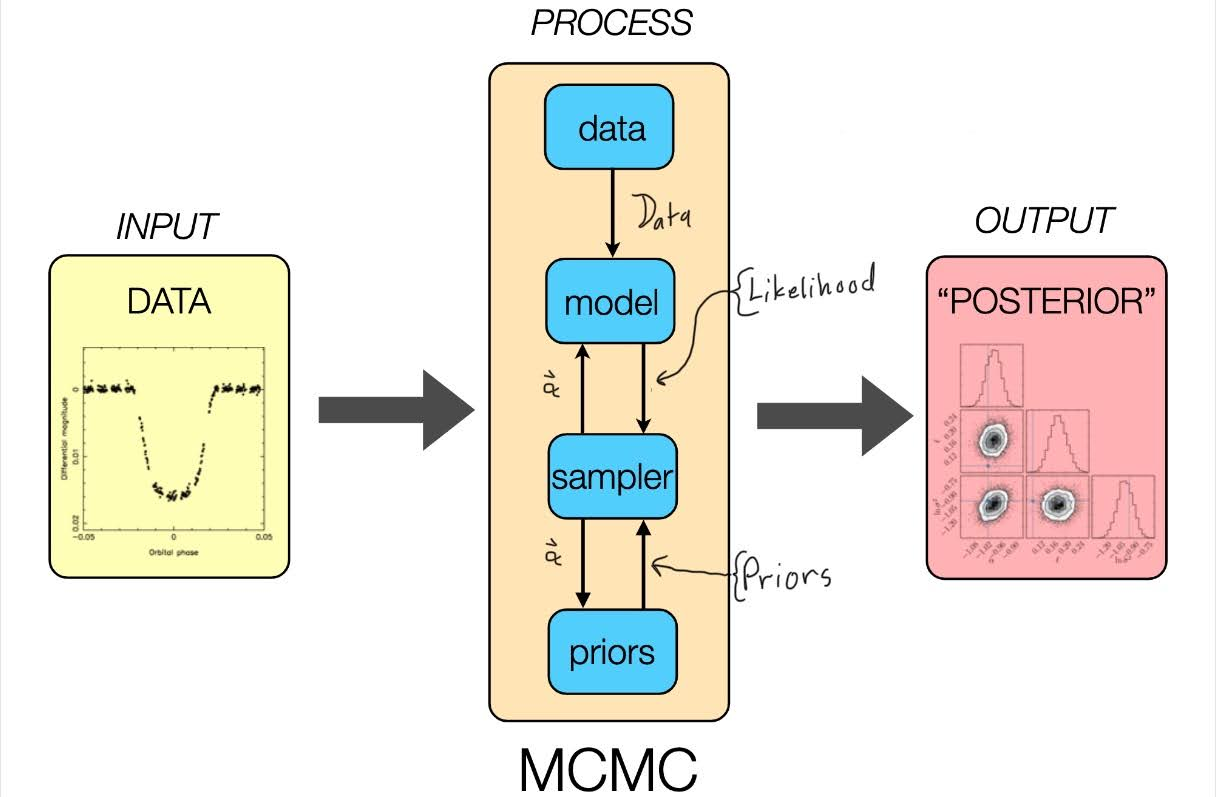
\includegraphics[width=0.9\linewidth]{mcmc-diag-kipping}
	\caption{MCMC Process - Taken from MCMC lecture by David Kipping \cite{Kipping_2016}}
\end{figure}

The MCMC process takes in some data set. Then it goes through a number of iterations of the process; the sampler provides parameter values out of the prior distributions to the model, which uses the data and the likelihood to provide an updated value for the parameter, which is used to generate the posterior. After enough of these steps, the posterior should model fairly well the distributions the unknown parameters should take so that the model best fits the data.

\newpage

\begin{center}
	\textbf{Metropolis Algorithm}
\end{center}
\begin{figure}[H]
	\begin{subfigure}{0.5\textwidth}
		\centering
		Markov Walk
		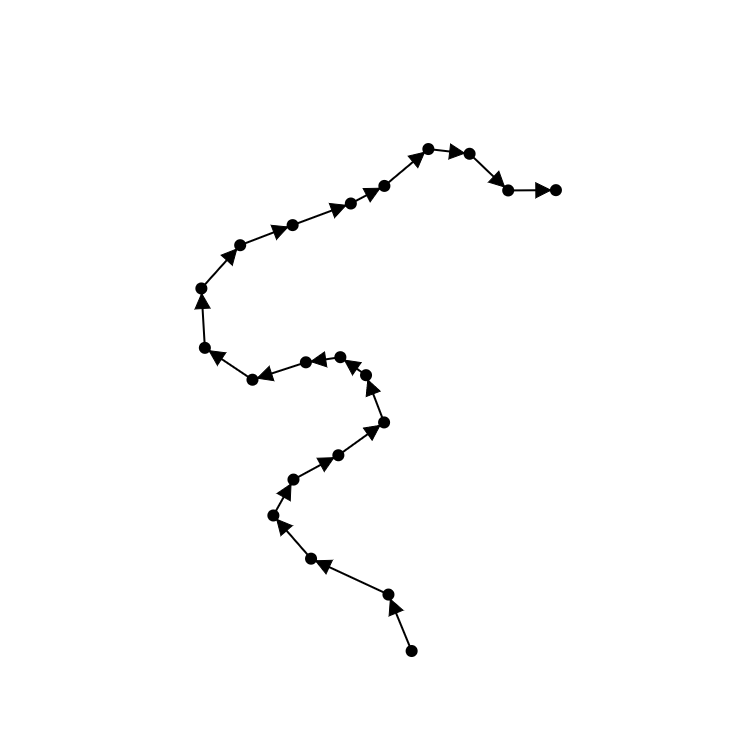
\includegraphics[width=\linewidth]{mcmc-start}
		\caption{Markov chain beginning walk}
	\end{subfigure}\hspace{\fill}
	\begin{subfigure}{0.5\textwidth}
		\centering
		Finding parameter distribution
		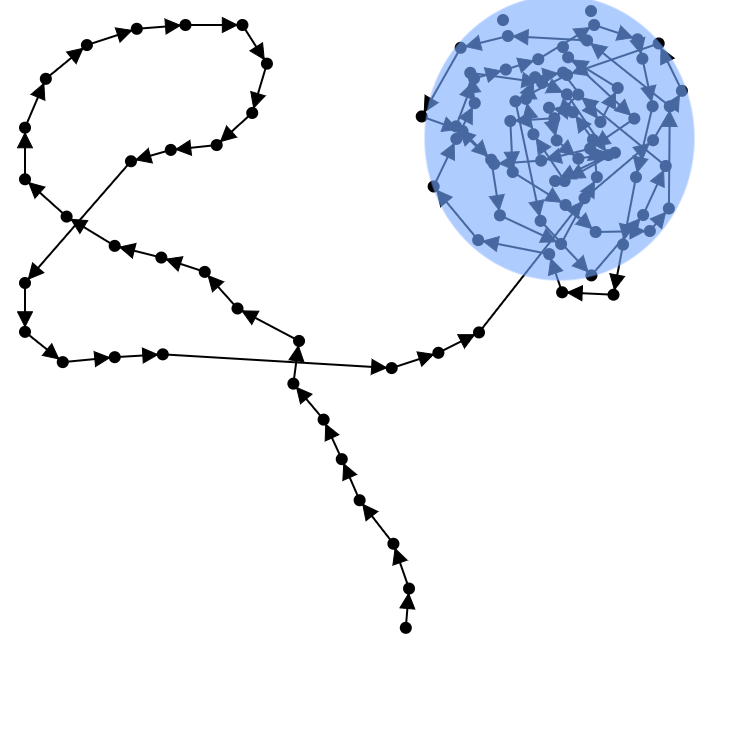
\includegraphics[width=\linewidth]{mcmc-circling}
		\caption{Eventually, it finds the distribution space}
	\end{subfigure}
\end{figure}

The algorithm for each step in the cahin, used by Dean et al.\ and continued here, is the Metropolis algorithm. It repeats a few basic steps:

\begin{itemize}
	\item Make a new parameter guess from priors
	\item Determine effectiveness of guess using likelihood.
	      \begin{itemize}
		      \item If the likelihood is better than the previous guess, that becomes the next state in the chain
		      \item If not, the algorithm tries a new guess. (Note: This re-guess is calculated halfway between the previous guess and missed guess in Metropolis-Hastings modification to the alg.)
	      \end{itemize}
	\item Use the new step as the starting point
\end{itemize}

As seen above, it begins via a rather random walk, slowly approaching the actual distribution zone for the parameter for the data. Once it reaches it, it generates more and more points in this zone, creating a good approximation for the parameter's actual distribution.
Notice that this leaves us with a pretty good set of points in the distribution, but having an unhelpful tail of values that were part of finding it. So, part of the MCMC process is to run the chain, but cut off a portion of it's beginning to avoid including the tail in the used distribution.

\newpage

\section {Comparison}

\subsubsection{Setup}

The known parameters for the existing models were gathered from historical data, inference of other variables, and the result of some formula. For a full derivation, see the article by Dean et. al.\ \cite{Dean1304}
For the unknown parameters, MCMC simulations are run to estimate based on data. For each model, we have set up the same process, and will examine the same datasets.
The full dataset was obtained from a Royal Society paper \cite{Sun_Xu_et_al_2019_dataset}, and contains the same death data by city as the original Dean et al.\ work. The datasets used here are deaths per day in Barcelona (1490), Florence (1400), and Malta (1813). These were chosen from the original 9 datasets tested in Dean et al.\ to be representative of comparative performance. Barcelona was chosen, as it performed very well with the Human-Ecto model and was worse than the pneomonic with the existing rat model. Malta and Florence were chosen because all previous models struggled to fit well.

Each MCMC simulation took 3 samplings of 180,000 iterations with 80,000 burn-in steps and a thinning of 10. This follows the same process as was conducted by Dean et al.

In the following graphs, the black data points are recorded deaths pre day in the given data set. The red line represents the model output, and the pink outline represents the model's 95\% C.I.

\newpage

\subsubsection{Barcelona}
For deaths in Barcelona in 1490:

\begin{center}
	\textbf{Barcelona - 1490}
\end{center}
\begin{figure}[H]
	\begin{subfigure}{0.5\textwidth}
		\centering
		Pneumonic Model
		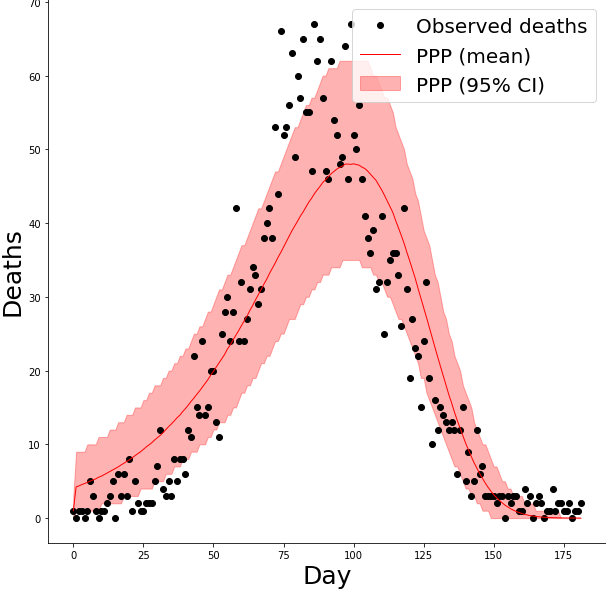
\includegraphics[width=\linewidth]{pneum/barcelona}
	\end{subfigure}\hspace{\fill}
	\begin{subfigure}{0.5\textwidth}
		\centering
		Keeling-Gilligan RFT Model
		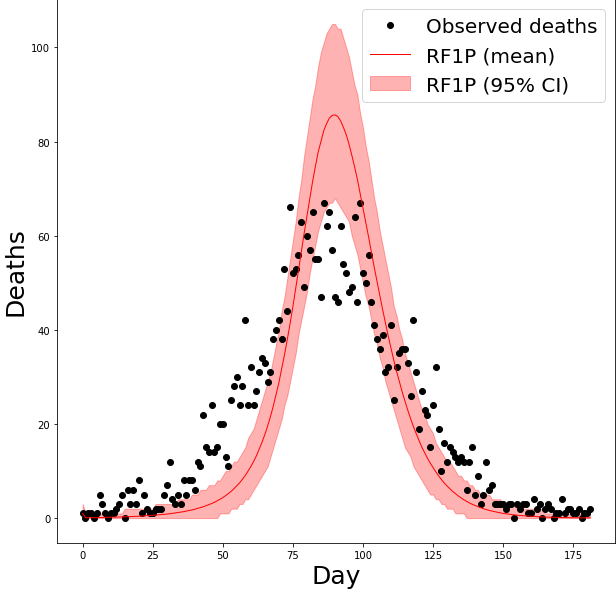
\includegraphics[width=\linewidth]{rats1/barcelona}
	\end{subfigure}
	\begin{subfigure}{0.5\textwidth}
		\centering
		Human-Ecto Model
		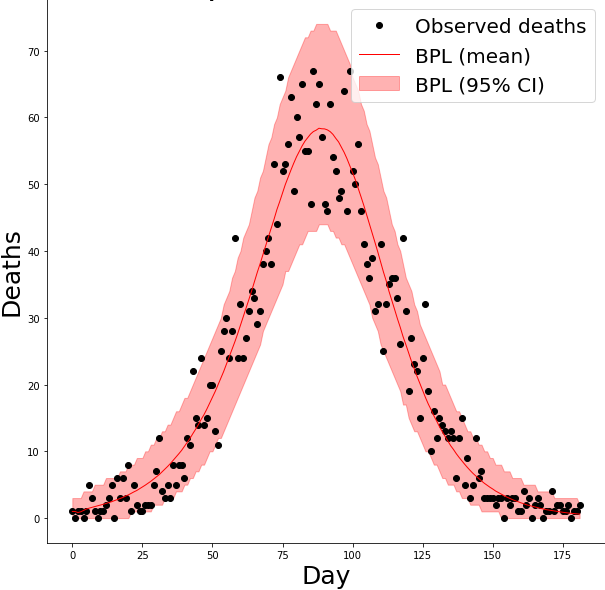
\includegraphics[width=\linewidth]{h_ecto/barcelona}
	\end{subfigure}\hspace{\fill}
	\begin{subfigure}{0.5\textwidth}
		\centering
		Lynch-Oster RFT Model
		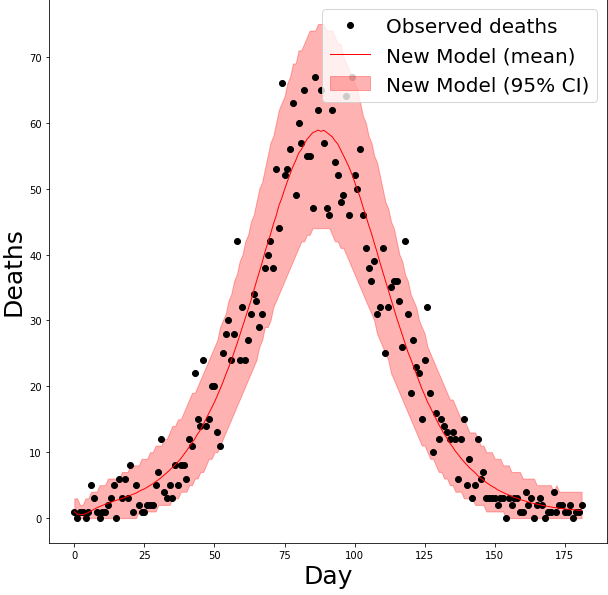
\includegraphics[width=\linewidth]{rats2/barcelona}
	\end{subfigure}
	\caption{Barcelona - 1490. Spans 182 days, Peaks at 67 deaths.}
\end{figure}

\newpage

\subsubsection{Malta}
For deaths in Malta in 1813:

\begin{center}
	\textbf{Malta - 1813}
\end{center}
\begin{figure}[H]
	\begin{subfigure}{0.5\textwidth}
		\centering
		Pneumonic Model
		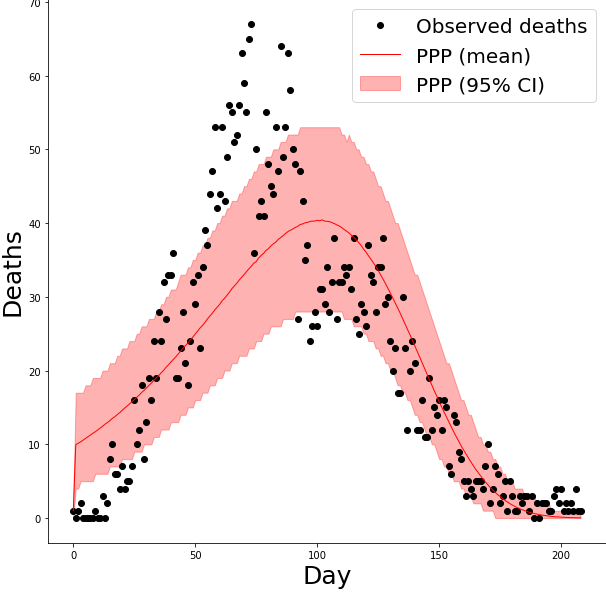
\includegraphics[width=\linewidth]{pneum/malta}
	\end{subfigure}\hspace{\fill}
	\begin{subfigure}{0.5\textwidth}
		\centering
		Keeling-Gilligan RFT Model
		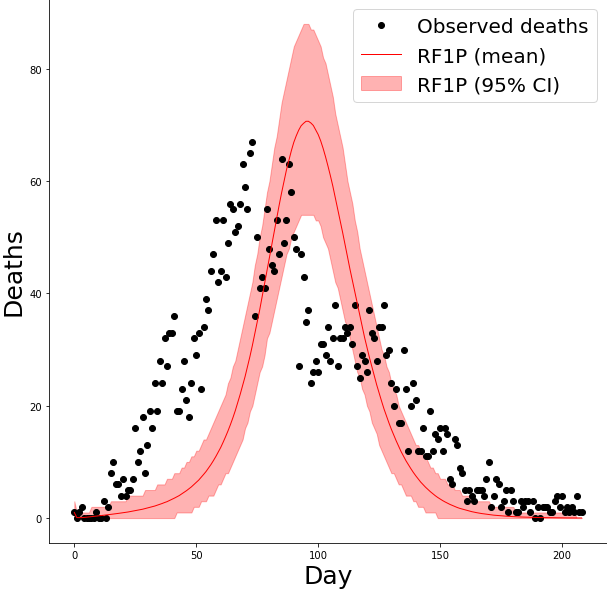
\includegraphics[width=\linewidth]{rats1/malta}
	\end{subfigure}
	\begin{subfigure}{0.5\textwidth}
		\centering
		Human-Ecto Model
		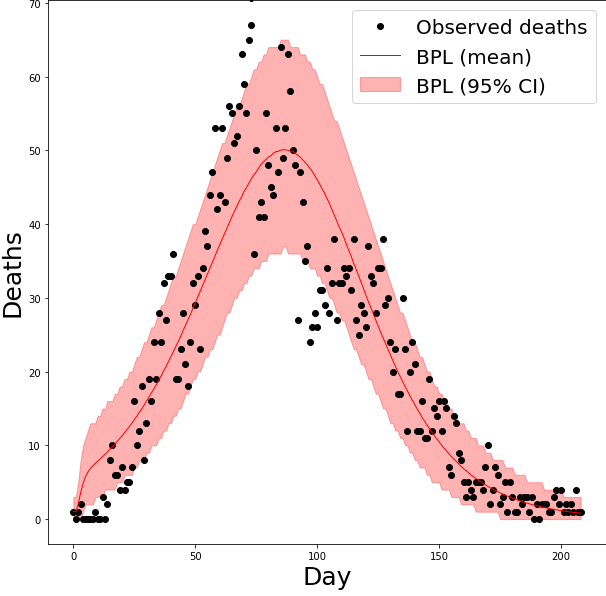
\includegraphics[width=\linewidth]{h_ecto/malta}
	\end{subfigure}\hspace{\fill}
	\begin{subfigure}{0.5\textwidth}
		\centering
		Lynch-Oster RFT Model
		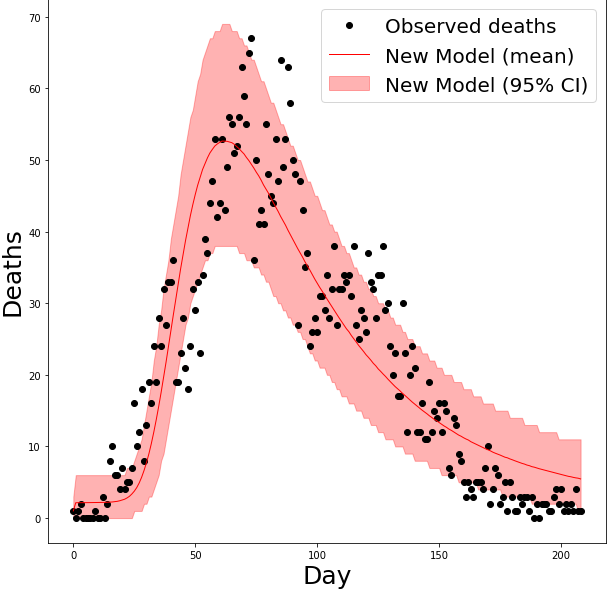
\includegraphics[width=\linewidth]{rats2/malta}
	\end{subfigure}
	\caption{Malta - 1813. Spans 209 days, Peaks at 67 deaths}
\end{figure}


\newpage

\subsubsection{Florence}
For deaths in Florence in 1400:

\begin{center}
	\textbf{Florence - 1400}
\end{center}
\begin{figure}[H]
	\begin{subfigure}{0.5\textwidth}
		\centering
		Pneumonic Model
		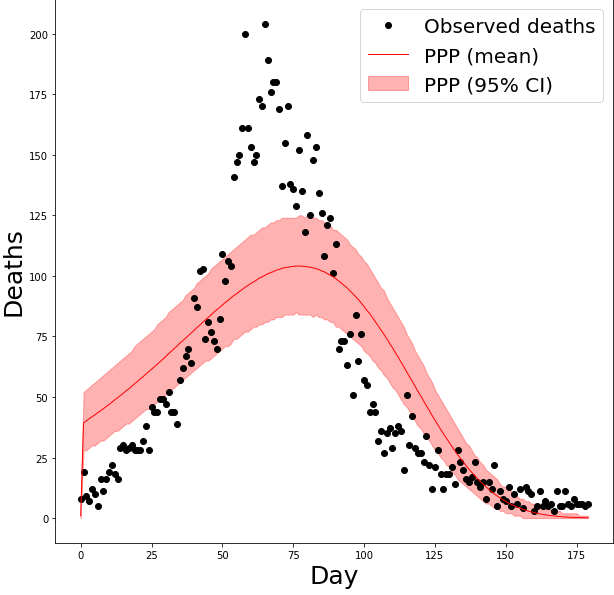
\includegraphics[width=\linewidth]{pneum/florence}
	\end{subfigure}\hspace{\fill}
	\begin{subfigure}{0.5\textwidth}
		\centering
		Keeling-Gilligan RFT Model
		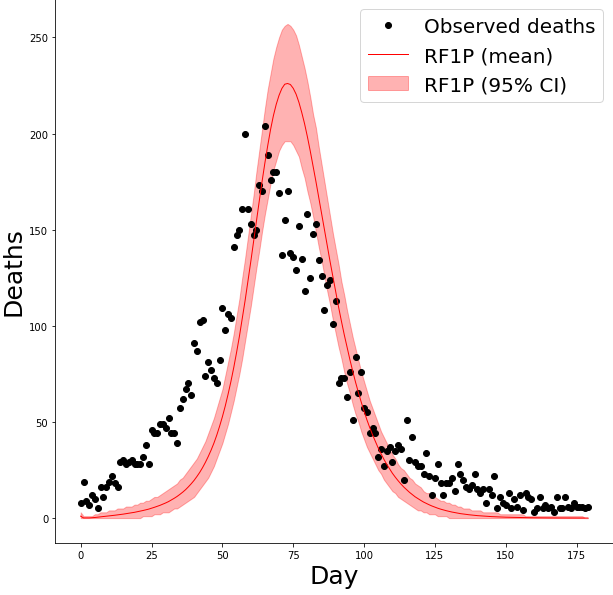
\includegraphics[width=\linewidth]{rats1/florence}
	\end{subfigure}
	\begin{subfigure}{0.5\textwidth}
		\centering
		Human-Ecto Model
		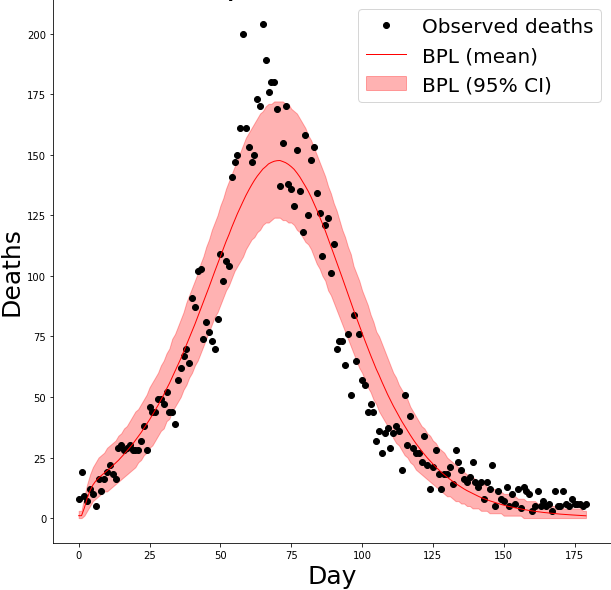
\includegraphics[width=\linewidth]{h_ecto/florence}
	\end{subfigure}\hspace{\fill}
	\begin{subfigure}{0.5\textwidth}
		\centering
		Lynch-Oster RFT Model
		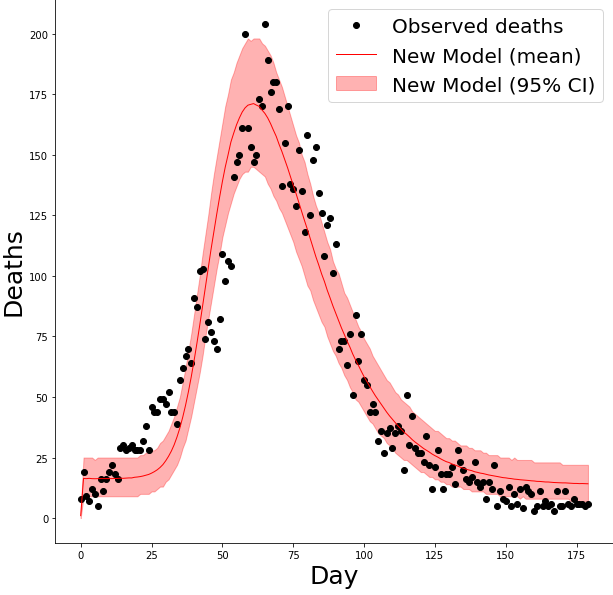
\includegraphics[width=\linewidth]{rats2/florence}
	\end{subfigure}
	\caption{Florence - 1400. Spans 180 days, Peaks at 204 deaths.}
\end{figure}

\newpage


\subsubsection{Summary}

The effectiveness of each model was measured using the Bayesian Information criterion (BIC). Here are the corresponding values for each dataset, sorted from best to worst fitting.

\begin{table}[H]
	\begin{center}
		\begin{tabular}{|l|l|l|}
			\hline
			\textbf{Dataset} & \textbf{Model}       & \textbf{BIC} \\ \hline
			Barcelona        & Human-Ecto           & 1945         \\ \cline{2-3}
			                 & Lynch-Oster RFT      & 2002         \\ \cline{2-3}
			                 & Pneumonic            & 2411         \\ \cline{2-3}
			                 & Keeling-Gilligan RFT & 3392         \\ \hline
			Malta            & Human-Ecto           & 1945         \\ \cline{2-3}
			                 & Lynch-Oster RFT      & 2491         \\ \cline{2-3}
			                 & Pneumonic            & 3806         \\ \cline{2-3}
			                 & Rat-flea 1           & 8274         \\ \hline
			Florence         & Lynch-Oster RFT      & 2375         \\ \cline{2-3}
			                 & Human-Ecto           & 2780         \\ \cline{2-3}
			                 & Pneumonic            & 4660         \\ \cline{2-3}
			                 & Keeling-Gilligan RFT & 15547        \\ \hline
		\end{tabular}
	\end{center}
	\caption{BIC values per data set. A lower value indicates a better fit.}
\end{table}

The accuracy of the mean prediction of each model relative to the data was measured using the Root Mean Square Error (RMSE). Here are the corresponding values for each dataset, sorted from least to most error.

\begin{table}[H]
	\begin{center}
		\begin{tabular}{|l|l|l|}
			\hline
			\textbf{Dataset} & \textbf{Model}       & \textbf{RMSE} \\ \hline
			Barcelona        & Lynch-Oster RFT      & 4.8           \\ \cline{2-3}
			                 & Human-Ecto           & 4.9           \\ \cline{2-3}
			                 & Pneumonic            & 8.1           \\ \cline{2-3}
			                 & Keeling-Gilligan RFT & 10.6          \\ \hline
			Malta            & Human-Ecto           & 7.4           \\ \cline{2-3}
			                 & Lynch-Oster RFT      & 7.8           \\ \cline{2-3}
			                 & Pneumonic            & 10.0          \\ \cline{2-3}
			                 & Keeling-Gilligan RFT & 17.6          \\ \hline
			Florence         & Human-Ecto           & 15.6          \\ \cline{2-3}
			                 & Lynch-Oster RFT      & 16.9          \\ \cline{2-3}
			                 & Pneumonic            & 31.3          \\ \cline{2-3}
			                 & Keeling-Gilligan RFT & 32.7          \\ \hline
		\end{tabular}
	\end{center}
	\caption{RMSE values per data set. A lower value indicates a better prediction.}
\end{table}


\newpage
\section {Discussion}
\vspace{-0.3cm}
\subsection{Interpreting the Results}
\vspace{-0.3cm}
The BIC measures how well the model with the given posterior parameter distributions fits the data. It tends to penalize models with more estimated parameters in order to avoid overfitting, but overall gives a good effectiveness of fit.
The RMSE measures how close the mean model prediction gets to accounting for the data. This better explains how well this model works in practice, when used used in a prediction setting.

Looking at these metrics, the Lynch-Oster model performed quite well. In each case, it was a better fit than the pneumonic and Keelin-Gilligan rat model. It performed about on par with the human-ecto model in Barcelona, and outperformed it in Florence. The model means were comparable, though the human-ecto model outperformed slightly.

\vspace{-0.3cm}

\subsection{Conclusions}
\vspace{-0.3cm}
While there is no clear winner when looking at the Human-ectoparasite and the Lynch-Oster models for plague spread, it's clear the new rat model brings solid evidence that the rat-based plague interpretation is certainly plausible.

\vspace{-0.3cm}
\subsection{Future Work}
\vspace{-0.3cm}
These results then spur on additional research. There are a few ways this could be improved.

The first is to fit the models against more data. While one model might not perform best overall, it could at least give a better picture of what types of plague were active where and when.

Another improvement to this research is to update the technologies used. The most up-to-date version of the PyMC library supports Python 3 and a new NUTS algorithm for Markov chains. NUTS models hamiltonian physics to get a quicker layout of the distribution space per markov step. It often converges more accurately and quickly with a larger number of parameters when compared to Metropolis-Hastings.

There is also more work that could be done in the fitting process. Currently, each model is run independently in Jupyter notebooks with most of the fitting process copied. This is adapted from the methods used in the Dean et al.\ work. It would be beneficial for future model fitting to streamline the process to allow easily swapping out models, data, and graphing styles.

A generalization of this process could allow researchers to quickly test the efficacy of new models against existing ones, and come up with better comparisons. In addition, future spreadable diseases could be understood more quickly. Not only could the method of transmission be approached more quickly, but parameters related to the spread could be estimated. Then, given a fitted model and distributions for parameters, efforts to prevent the spread could be tested and the effectiveness of different methods realized before a significant portion of the population becomes infected.

\pagebreak

\bibliography{References.bib}
\bibliographystyle{plain}

\end{document}